\documentclass{jsarticle}
\usepackage{color}
\usepackage{bm}
\usepackage{mathrsfs}
\usepackage[height=26cm,width=16cm]{geometry} 
\usepackage{amsmath}
\usepackage{cases}
\usepackage[dvipdfmx]{graphicx}
\title{電磁気学}
\graphicspath{{./image/}}

\begin{document}

\section{電場}
	\subsection{無限電場}
		・無限に長い直線上に電荷密度λで電荷が分布\\
		→Pに作る電場は?\\
		領域ΔSにおける電荷\\
		\[
			=\lambda \Delta S
		\]
		→Pに作る電場は
		\[
			\frac{\lambda \Delta S}{4\pi \varepsilon_0}\frac{1}{(\sqrt{r^2+s^2})^2}
		\]
		\[
			E_\perp =\frac{\lambda \Delta S}{4\pi \varepsilon_0}\frac{1}{r^2+s^2}\frac{r}{\sqrt{r^2+s^2}}=\frac{\lambda \Delta S}{4\pi \varepsilon_0}\frac{r}{(\sqrt{r^2+s^2})^3}
		\]
		線状全ての寄与を与える→全ての$E_\perp$を積分
		\[
			E=\int^\infty_{-\infty} \frac{\lambda}{4 \pi \varepsilon_0} \frac{r}{(r^2+s^2)^{\frac{3}{2}}} ds
		\]
		\[
			-\infty<S<\infty → -\frac{\pi}{2}<\theta <\frac{\pi}{2}
		\]
		\begin{eqnarray}
			S=r\tan \theta \\
			dS=r\sec^2\theta d\theta
		\end{eqnarray}
		\[
			s^2+r^2=r^2(1+\tan^2 \theta)=\frac{r^2}{\cos^2\theta}=r^2\sec^2\theta
		\]
		\[
			E=\int^{\frac{\pi}{2}}_{-\frac{\pi}{2}}\frac{\lambda}{4\pi\varepsilon_0}\frac{r^2\sec^2\theta}{r^3\sec^3\theta}d\theta=\frac{\lambda}{4 \pi \varepsilon_0r}\int^{\frac{\pi}{2}}_{-\frac{\pi}{2}}\cos\theta d\theta=\frac{\lambda}{2 \pi \varepsilon_0r}
		\]
		\begin{minipage}{0.5\hsize}	
		\begin{center}
			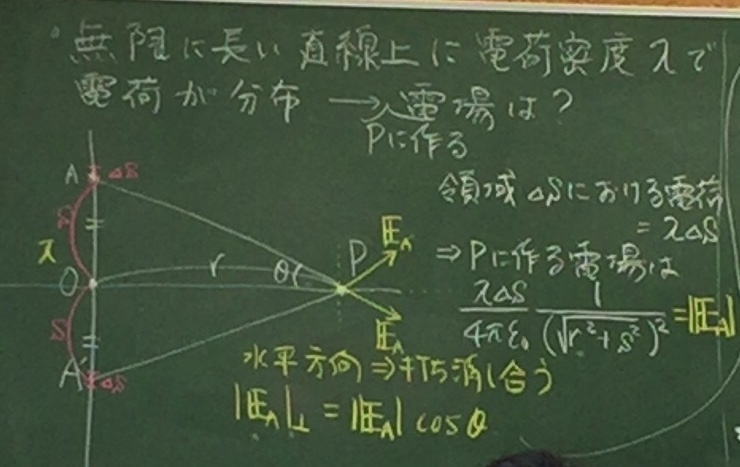
\includegraphics[width=7cm]{5_10_1.JPG}
		\end{center}
		\end{minipage}
		\begin{minipage}{0.5\hsize}	
		\begin{center}
			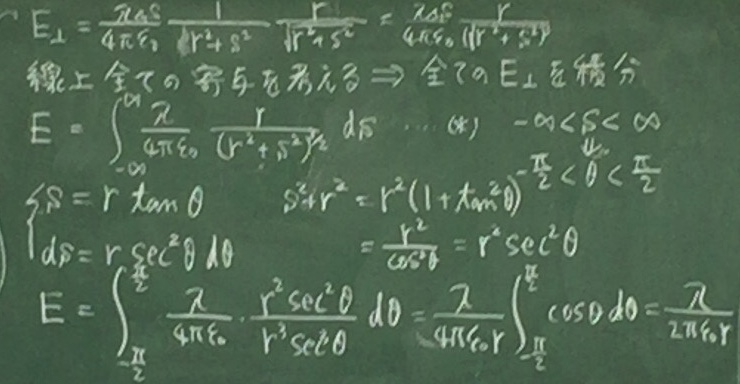
\includegraphics[width=7cm]{5_10_2.JPG}
		\end{center}
		\end{minipage}
	\subsection{電気力線}
		・電場の様子を向き、強さで逗子\\
		・正(負)の電荷があると線の向き外(内)向き\\
		\begin{center}
			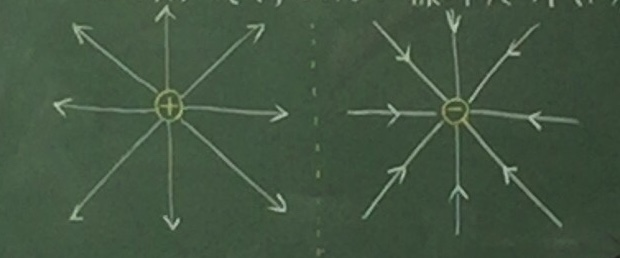
\includegraphics[width=7cm]{5_10_3.JPG}
		\end{center}
		微小面積ΔSをΔNの力線が貫いているとき、\\
		\begin{center}
			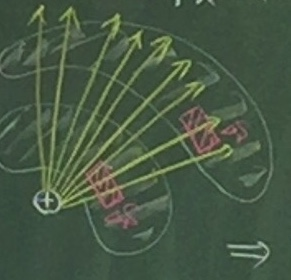
\includegraphics[width=5cm]{5_10_4.JPG}
		\end{center}
		$電気力線の密度
			\frac{\Delta N}{\Delta S}$
		同じΔSであっても電荷に近い方がΔNは大きい\\
		→電場の強さ$\propto$電気力線の密度\\
		・電荷を中心、半径rの球の表面積$S=4\pi r^2$\\
		電荷から出る力線の本数をNとする\\
		電気力線の密度:
		\[\frac{N}{4\pi r^2}
		\]
		電場の強度:
		\[
			\frac{q}{4\pi \varepsilon_0 r^2}
		\]
		・正負ついの電荷がある場合(絶対値は等しい)
		\begin{center}
			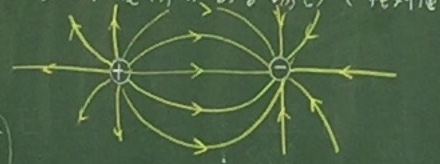
\includegraphics[width=7cm]{5_10_5.JPG}
		\end{center}
		直線上に等間隔に$-q,2q,-q$と電荷が並ぶ場合($q>0$)\\
		同じ微小領域を貫く力線の本数に差がある\\
		\begin{center}
			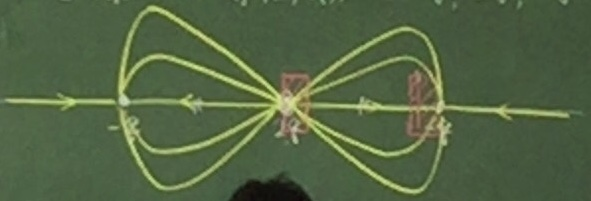
\includegraphics[width=7cm]{5_10_6.JPG}
		\end{center}
	\subsection{ガウスの法則}
		{\Large・ある閉曲面Sの内側に電荷がある場合}\\
		力線は全て内側→外側へ出る\\
		Sを貫く力線の本数→電荷の大きさのみに依存\\
		\begin{minipage}{0.5\hsize}	
		\begin{center}
			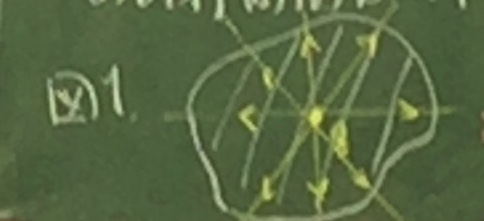
\includegraphics[width=7cm]{5_10_7.JPG}
		\end{center}
		\end{minipage}
		\begin{minipage}{0.5\hsize}	
		\begin{center}
			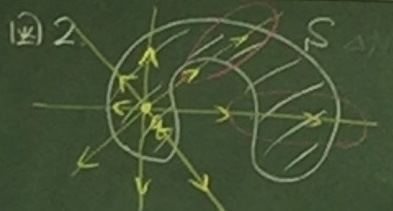
\includegraphics[width=7cm]{5_10_8.JPG}
		\end{center}
		\end{minipage}
		Sから出た力線が再びSに入り、また出て行く\\
		・外から入り込む→負\\
		・外へ出て行く  →正\\
		よって、赤で囲った部分は0→力線の本数の代数和\\
		Sを貫く電気力線の代数和は電荷の大きさのみに依存→難しく考えすぎるな\\
		\begin{center}
			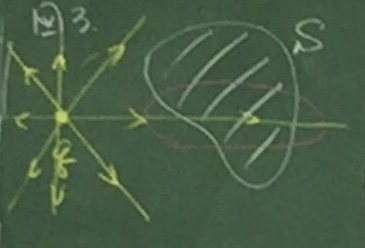
\includegraphics[width=7cm]{5_10_9.JPG}
		\end{center}
		{\Large ・電荷が閉曲面の外}\\
		Sを貫く力線の代数和は{\Large 0}\\
		{\Large ・閉曲面の中に電荷がある}\\
		微小領域$\Delta S$を考える\\
		$\Delta S$を貫く電気力線の本数$\Delta N$、力線に垂直な面$\Delta S'$、$\Delta S$の法線ベクトル$\bf r$\\
		\[
			\Delta S'=\Delta S \cos \theta
		\]
		\begin{center}
			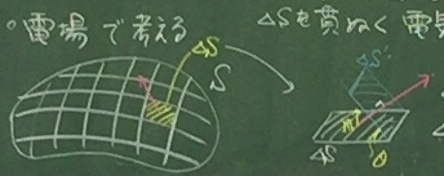
\includegraphics[width=7cm]{5_10_10.JPG}
		\end{center}
		電気力線の密度:
		\[
			\frac{\Delta N}{\Delta S'}=\frac{\Delta N}{\Delta S\cos \theta}=k|\bm{E}|
		\]
		kは比例定数
		\[
			\Delta N=k|\bf E|\cos \theta \Delta S
		\]
		\[
			|\bm{E}|\cos \theta=\bm{E}\cdot \bm{n}=E_n
		\]
		$E_n$:$|\bf{E}|$を領域$\Delta S$に垂直な方向へ射影\\
		閉曲面内全ての$\Delta S$を足し合わせると、Sを貫く力線の総和となる\\
		\[
			N=k\sum (\bm{E}\cdot \bm{n})\Delta S
		\]
		S内に電荷がない場合→
		\[
			k\sum (\bm{E}\cdot \bm{n})\Delta S=0
		\]
		$\Delta S→0$の極限を考える
		\[
			\int_S {\bm{E}(\bm{r})\cdot \bm{n}(\bm{r})}dS = 0
		\]
		面積分\\
		局面の一部が平面の場合、直交座標$(x,y)$で考えることができる$dS=dxdy$
		\[
			\int\int E_n(x,y)dxdy
		\]
\end{document}





